
%% bare_conf.tex
%% V1.3
%% 2007/01/11
%% by Michael Shell
%% See:
%% http://www.michaelshell.org/
%% for current contact information.
%%
%% This is a skeleton file demonstrating the use of IEEEtran.cls
%% (requires IEEEtran.cls version 1.7 or later) with an IEEE conference paper.
%%
%% Support sites:
%% http://www.michaelshell.org/tex/ieeetran/
%% http://www.ctan.org/tex-archive/macros/latex/contrib/IEEEtran/
%% and
%% http://www.ieee.org/

%%*************************************************************************
%% Legal Notice:
%% This code is offered as-is without any warranty either expressed or
%% implied; without even the implied warranty of MERCHANTABILITY or
%% FITNESS FOR A PARTICULAR PURPOSE! 
%% User assumes all risk.
%% In no event shall IEEE or any contributor to this code be liable for
%% any damages or losses, including, but not limited to, incidental,
%% consequential, or any other damages, resulting from the use or misuse
%% of any information contained here.
%%
%% All comments are the opinions of their respective authors and are not
%% necessarily endorsed by the IEEE.
%%
%% This work is distributed under the LaTeX Project Public License (LPPL)
%% ( http://www.latex-project.org/ ) version 1.3, and may be freely used,
%% distributed and modified. A copy of the LPPL, version 1.3, is included
%% in the base LaTeX documentation of all distributions of LaTeX released
%% 2003/12/01 or later.
%% Retain all contribution notices and credits.
%% ** Modified files should be clearly indicated as such, including  **
%% ** renaming them and changing author support contact information. **
%%
%% File list of work: IEEEtran.cls, IEEEtran_HOWTO.pdf, bare_adv.tex,
%%                    bare_conf.tex, bare_jrnl.tex, bare_jrnl_compsoc.tex
%%*************************************************************************

% *** Authors should verify (and, if needed, correct) their LaTeX system  ***
% *** with the testflow diagnostic prior to trusting their LaTeX platform ***
% *** with production work. IEEE's font choices can trigger bugs that do  ***
% *** not appear when using other class files.                            ***
% The testflow support page is at:
% http://www.michaelshell.org/tex/testflow/



% Note that the a4paper option is mainly intended so that authors in
% countries using A4 can easily print to A4 and see how their papers will
% look in print - the typesetting of the document will not typically be
% affected with changes in paper size (but the bottom and side margins will).
% Use the testflow package mentioned above to verify correct handling of
% both paper sizes by the user's LaTeX system.
%
% Also note that the "draftcls" or "draftclsnofoot", not "draft", option
% should be used if it is desired that the figures are to be displayed in
% draft mode.
%
\documentclass[conference]{IEEEtran}
% Add the compsoc option for Computer Society conferences.
%
% If IEEEtran.cls has not been installed into the LaTeX system files,
% manually specify the path to it like:
% \documentclass[conference]{../sty/IEEEtran}





% Some very useful LaTeX packages include:
% (uncomment the ones you want to load)


% *** MISC UTILITY PACKAGES ***
%
%\usepackage{ifpdf}
% Heiko Oberdiek's ifpdf.sty is very useful if you need conditional
% compilation based on whether the output is pdf or dvi.
% usage:
% \ifpdf
%   % pdf code
% \else
%   % dvi code
% \fi
% The latest version of ifpdf.sty can be obtained from:
% http://www.ctan.org/tex-archive/macros/latex/contrib/oberdiek/
% Also, note that IEEEtran.cls V1.7 and later provides a builtin
% \ifCLASSINFOpdf conditional that works the same way.
% When switching from latex to pdflatex and vice-versa, the compiler may
% have to be run twice to clear warning/error messages.






% *** CITATION PACKAGES ***
%
%\usepackage{cite}
% cite.sty was written by Donald Arseneau
% V1.6 and later of IEEEtran pre-defines the format of the cite.sty package
% \cite{} output to follow that of IEEE. Loading the cite package will
% result in citation numbers being automatically sorted and properly
% "compressed/ranged". e.g., [1], [9], [2], [7], [5], [6] without using
% cite.sty will become [1], [2], [5]--[7], [9] using cite.sty. cite.sty's
% \cite will automatically add leading space, if needed. Use cite.sty's
% noadjust option (cite.sty V3.8 and later) if you want to turn this off.
% cite.sty is already installed on most LaTeX systems. Be sure and use
% version 4.0 (2003-05-27) and later if using hyperref.sty. cite.sty does
% not currently provide for hyperlinked citations.
% The latest version can be obtained at:
% http://www.ctan.org/tex-archive/macros/latex/contrib/cite/
% The documentation is contained in the cite.sty file itself.






% *** GRAPHICS RELATED PACKAGES ***

  \usepackage[dvips]{graphicx}
 \graphicspath{{../eps/}}

%
%\ifCLASSINFOpdf
  % \usepackage[pdftex]{graphicx}
  % declare the path(s) where your graphic files are
  % \graphicspath{{../pdf/}{../jpeg/}}
  % and their extensions so you won't have to specify these with
  % every instance of \includegraphics
  % \DeclareGraphicsExtensions{.pdf,.jpeg,.png}
%\else
  % or other class option (dvipsone, dvipdf, if not using dvips). graphicx
  % will default to the driver specified in the system graphics.cfg if no
  % driver is specified.
  % \usepackage[dvips]{graphicx}
  % declare the path(s) where your graphic files are
  \graphicspath{{../eps/}}
  % and their extensions so you won't have to specify these with
  % every instance of \includegraphics
  % \DeclareGraphicsExtensions{.eps}
%\fi
% graphicx was written by David Carlisle and Sebastian Rahtz. It is
% required if you want graphics, photos, etc. graphicx.sty is already
% installed on most LaTeX systems. The latest version and documentation can
% be obtained at: 
% http://www.ctan.org/tex-archive/macros/latex/required/graphics/
% Another good source of documentation is "Using Imported Graphics in
% LaTeX2e" by Keith Reckdahl which can be found as epslatex.ps or
% epslatex.pdf at: http://www.ctan.org/tex-archive/info/
%
% latex, and pdflatex in dvi mode, support graphics in encapsulated
% postscript (.eps) format. pdflatex in pdf mode supports graphics
% in .pdf, .jpeg, .png and .mps (metapost) formats. Users should ensure
% that all non-photo figures use a vector format (.eps, .pdf, .mps) and
% not a bitmapped formats (.jpeg, .png). IEEE frowns on bitmapped formats
% which can result in "jaggedy"/blurry rendering of lines and letters as
% well as large increases in file sizes.
%
% You can find documentation about the pdfTeX application at:
% http://www.tug.org/applications/pdftex





% *** MATH PACKAGES ***
%
%\usepackage[cmex10]{amsmath}
% A popular package from the American Mathematical Society that provides
% many useful and powerful commands for dealing with mathematics. If using
% it, be sure to load this package with the cmex10 option to ensure that
% only type 1 fonts will utilized at all point sizes. Without this option,
% it is possible that some math symbols, particularly those within
% footnotes, will be rendered in bitmap form which will result in a
% document that can not be IEEE Xplore compliant!
%
% Also, note that the amsmath package sets \interdisplaylinepenalty to 10000
% thus preventing page breaks from occurring within multiline equations. Use:
%\interdisplaylinepenalty=2500
% after loading amsmath to restore such page breaks as IEEEtran.cls normally
% does. amsmath.sty is already installed on most LaTeX systems. The latest
% version and documentation can be obtained at:
% http://www.ctan.org/tex-archive/macros/latex/required/amslatex/math/





% *** SPECIALIZED LIST PACKAGES ***
%
%\usepackage{algorithmic}
% algorithmic.sty was written by Peter Williams and Rogerio Brito.
% This package provides an algorithmic environment fo describing algorithms.
% You can use the algorithmic environment in-text or within a figure
% environment to provide for a floating algorithm. Do NOT use the algorithm
% floating environment provided by algorithm.sty (by the same authors) or
% algorithm2e.sty (by Christophe Fiorio) as IEEE does not use dedicated
% algorithm float types and packages that provide these will not provide
% correct IEEE style captions. The latest version and documentation of
% algorithmic.sty can be obtained at:
% http://www.ctan.org/tex-archive/macros/latex/contrib/algorithms/
% There is also a support site at:
% http://algorithms.berlios.de/index.html
% Also of interest may be the (relatively newer and more customizable)
% algorithmicx.sty package by Szasz Janos:
% http://www.ctan.org/tex-archive/macros/latex/contrib/algorithmicx/




% *** ALIGNMENT PACKAGES ***
%
%\usepackage{array}
% Frank Mittelbach's and David Carlisle's array.sty patches and improves
% the standard LaTeX2e array and tabular environments to provide better
% appearance and additional user controls. As the default LaTeX2e table
% generation code is lacking to the point of almost being broken with
% respect to the quality of the end results, all users are strongly
% advised to use an enhanced (at the very least that provided by array.sty)
% set of table tools. array.sty is already installed on most systems. The
% latest version and documentation can be obtained at:
% http://www.ctan.org/tex-archive/macros/latex/required/tools/


%\usepackage{mdwmath}
%\usepackage{mdwtab}
% Also highly recommended is Mark Wooding's extremely powerful MDW tools,
% especially mdwmath.sty and mdwtab.sty which are used to format equations
% and tables, respectively. The MDWtools set is already installed on most
% LaTeX systems. The lastest version and documentation is available at:
% http://www.ctan.org/tex-archive/macros/latex/contrib/mdwtools/


% IEEEtran contains the IEEEeqnarray family of commands that can be used to
% generate multiline equations as well as matrices, tables, etc., of high
% quality.


%\usepackage{eqparbox}
% Also of notable interest is Scott Pakin's eqparbox package for creating
% (automatically sized) equal width boxes - aka "natural width parboxes".
% Available at:
% http://www.ctan.org/tex-archive/macros/latex/contrib/eqparbox/





% *** SUBFIGURE PACKAGES ***
%\usepackage[tight,footnotesize]{subfigure}
% subfigure.sty was written by Steven Douglas Cochran. This package makes it
% easy to put subfigures in your figures. e.g., "Figure 1a and 1b". For IEEE
% work, it is a good idea to load it with the tight package option to reduce
% the amount of white space around the subfigures. subfigure.sty is already
% installed on most LaTeX systems. The latest version and documentation can
% be obtained at:
% http://www.ctan.org/tex-archive/obsolete/macros/latex/contrib/subfigure/
% subfigure.sty has been superceeded by subfig.sty.



%\usepackage[caption=false]{caption}
%\usepackage[font=footnotesize]{subfig}
% subfig.sty, also written by Steven Douglas Cochran, is the modern
% replacement for subfigure.sty. However, subfig.sty requires and
% automatically loads Axel Sommerfeldt's caption.sty which will override
% IEEEtran.cls handling of captions and this will result in nonIEEE style
% figure/table captions. To prevent this problem, be sure and preload
% caption.sty with its "caption=false" package option. This is will preserve
% IEEEtran.cls handing of captions. Version 1.3 (2005/06/28) and later 
% (recommended due to many improvements over 1.2) of subfig.sty supports
% the caption=false option directly:
%\usepackage[caption=false,font=footnotesize]{subfig}
%
% The latest version and documentation can be obtained at:
% http://www.ctan.org/tex-archive/macros/latex/contrib/subfig/
% The latest version and documentation of caption.sty can be obtained at:
% http://www.ctan.org/tex-archive/macros/latex/contrib/caption/




% *** FLOAT PACKAGES ***
%
%\usepackage{fixltx2e}
% fixltx2e, the successor to the earlier fix2col.sty, was written by
% Frank Mittelbach and David Carlisle. This package corrects a few problems
% in the LaTeX2e kernel, the most notable of which is that in current
% LaTeX2e releases, the ordering of single and double column floats is not
% guaranteed to be preserved. Thus, an unpatched LaTeX2e can allow a
% single column figure to be placed prior to an earlier double column
% figure. The latest version and documentation can be found at:
% http://www.ctan.org/tex-archive/macros/latex/base/



%\usepackage{stfloats}
% stfloats.sty was written by Sigitas Tolusis. This package gives LaTeX2e
% the ability to do double column floats at the bottom of the page as well
% as the top. (e.g., "\begin{figure*}[!b]" is not normally possible in
% LaTeX2e). It also provides a command:
%\fnbelowfloat
% to enable the placement of footnotes below bottom floats (the standard
% LaTeX2e kernel puts them above bottom floats). This is an invasive package
% which rewrites many portions of the LaTeX2e float routines. It may not work
% with other packages that modify the LaTeX2e float routines. The latest
% version and documentation can be obtained at:
% http://www.ctan.org/tex-archive/macros/latex/contrib/sttools/
% Documentation is contained in the stfloats.sty comments as well as in the
% presfull.pdf file. Do not use the stfloats baselinefloat ability as IEEE
% does not allow \baselineskip to stretch. Authors submitting work to the
% IEEE should note that IEEE rarely uses double column equations and
% that authors should try to avoid such use. Do not be tempted to use the
% cuted.sty or midfloat.sty packages (also by Sigitas Tolusis) as IEEE does
% not format its papers in such ways.





% *** PDF, URL AND HYPERLINK PACKAGES ***
%
%\usepackage{url}
% url.sty was written by Donald Arseneau. It provides better support for
% handling and breaking URLs. url.sty is already installed on most LaTeX
% systems. The latest version can be obtained at:
% http://www.ctan.org/tex-archive/macros/latex/contrib/misc/
% Read the url.sty source comments for usage information. Basically,
% \url{my_url_here}.

%*** for JSON document ***
\usepackage{minted}


%*** for listing environment ***
%\usepackage{listing}



% *** Do not adjust lengths that control margins, column widths, etc. ***
% *** Do not use packages that alter fonts (such as pslatex).         ***
% There should be no need to do such things with IEEEtran.cls V1.6 and later.
% (Unless specifically asked to do so by the journal or conference you plan
% to submit to, of course. )


% correct bad hyphenation here
\hyphenation{op-tical net-works semi-conduc-tor}


\begin{document}
%
% paper title
% can use linebreaks \\ within to get better formatting as desired
\title{ZeroVM enabled Content  Based Access Control for Swift Storage}


% author names and affiliations
% use a multiple column layout for up to three different
% affiliations

\author{
        %Jeffery~von Ronne,%~\IEEEmembership{UTSA}
        \IEEEauthorblockN{ Prosunjit Biswas~~~~Farhan Fatwa ~~~~ Dr. Ravi Sandhu } 
        \IEEEauthorblockA{Computer Science Department and Cloud and Big Data Laboratory\\
        The University of Texas at San Antonio\\
        eft434@my.utsa.edu~~~~farhan.patwa@utsa.edu ~~~~ravi.sandhu@utsa.edu}

}



% conference papers do not typically use \thanks and this command
% is locked out in conference mode. If really needed, such as for
% the acknowledgment of grants, issue a \IEEEoverridecommandlockouts
% after \documentclass

% for over three affiliations, or if they all won't fit within the width
% of the page, use this alternative format:
% 
%\author{\IEEEauthorblockN{Michael Shell\IEEEauthorrefmark{1},
%Homer Simpson\IEEEauthorrefmark{2},
%James Kirk\IEEEauthorrefmark{3}, 
%Montgomery Scott\IEEEauthorrefmark{3} and
%Eldon Tyrell\IEEEauthorrefmark{4}}
%\IEEEauthorblockA{\IEEEauthorrefmark{1}School of Electrical and Computer Engineering\\
%Georgia Institute of Technology,
%Atlanta, Georgia 30332--0250\\ Email: see http://www.michaelshell.org/contact.html}
%\IEEEauthorblockA{\IEEEauthorrefmark{2}Twentieth Century Fox, Springfield, USA\\
%Email: homer@thesimpsons.com}
%\IEEEauthorblockA{\IEEEauthorrefmark{3}Starfleet Academy, San Francisco, California 96678-2391\\
%Telephone: (800) 555--1212, Fax: (888) 555--1212}
%\IEEEauthorblockA{\IEEEauthorrefmark{4}Tyrell Inc., 123 Replicant Street, Los Angeles, California 90210--4321}}




% use for special paper notices
%\IEEEspecialpapernotice{(Invited Paper)}




% make the title area
\maketitle
\begin{abstract}

While Openstack swift facilitates storage and management of unlimited amount of data, with conventional cloud computing paradigm, for the purpose of  processing these enormous amount of data, it is required to be moved back and forth to the computing host exhausing significant cpu cycles and resulting serious I/O bottleneck. ZeroVM, a specially designed hypervisor for the cloud, eliminates unnecessary movement of data by enabling data local computing by virtue of uniquely designed applications called ZAP (zerovm application package) which facilitates computation around data inside swift storage.  This approach can enable swift customers to have sophisticated control over their data by specifying not only who can or cannot access their data, but also how much of the content can be accessed. Inspired by the fact, we are developing a zerovm application, that let data ownser specify access policy on the content of the data file and describe who can or cannot not access which portion of the data which is essentially more fine granined access control over the ACL based all/nothing access.  The prototype of our proposal  is implemented on JSON data formatted file. 

\end{abstract}
\section{Introduction}
OpenStack  Swift is a highly deployed open source cloud storage solution. With its unlimited storage capability, it is used to store any number of large / small objects through its  RESTful HTTP API. A user can  submit a GET request to download a  file and a PUT request to upload a file. But a fundamental problem in the cloud storage system is  that whenever data is required to be processed, it has to be moved to the computing hosts (ex. VM, EC2 instance) before computation and moved back to the original storage afterward which  results significant I/O overhead. 



ZeroVM \cite{zerovm}, an specially built hypervisor for the cloud promises to solve the problem of secure computation. This is an application vertualization technique based on google native client (NaCl) project \cite{nacl} which is able to run arbitrary ( and potentially malicious) code  and still provide security guarantee. Unlike existing solution like docker \cite{docker} which is also very exciting in its own merit, ZeroVM focuses more on fault isolation and secure computation. 


This new technoloy whenever integrated with  Swift storage, is able execute arbitrary application ( and potententially unsafe code) inside Swift cluster and process data locally. With its tight security guarante, ZeroVM assure both the data owner and storage provider  from potential security risks from completely untrusted application enabling data local in-storage computation. This new paradigm introduces whole lot of opportunities. For example, now it is possible to search data while data is in storage, look for patterns, or serve a file partially along with other exciting use cases like  running query for big data and  extracting salient customer pattern or product demand. 

The integration of these two new technologies also open up an exciting era for both cloud storage provider and cloud customer. From the perspective of storage provider, along with the storage they can also offer useful data processing applications  which may help customers to get better service and even save money which was spent due to the movement of data. From the customers perspective, they no longer need to provision large clusters that they used to use for the processing of the data.  

As an effort to develop a  ZeroVM application, we are proposing content based access control for object/files  stored in the object store.  we would enable Swift customers to specify who can access how much content of the  data. To give a concrete example, consider a hospital stores its patient record  in the object store. Now, these record files should be accessed differently by different personnels. For example, the doctor can see certain part  while the billing accoutant should see other part of the record. Our application would let the data owner specify policy expressing who can see which part of the data.

As  a prototype implementation, we would work with JSON formatted file because of several reasons. Firstly, JSON is gaining immense popularity due to its concise representation and easiness in human and machine readability. Secondly, industries are increasingly adopting JSON for internal data representation and data exchange format which is reflected by the facts that JSON  document database such as MongoDB(more accurately BSON, a modified version JSON) is now officially supported by the OpenStack cloud platform; Twitter latest API (v 1.1) supports only JSON and Youtube’s latest API (v 3) \cite{identityv3} recommend JSON as the default exchange format. Thirdly, we believe that JSON could be a easily adapted  for semi-structured / unstructured big data. 



\section{Background}

To keep the readers comfortable to our work, we would introduce  the concepts of Attribute Based Access Control (ABAC) model very briefly.

\subsection{Attribute Based Access Control}

Attribute-based access control defines a new access control paradigm whereby access rights are granted to users through the use of policies which combine attributes together. The policies can use any type of attributes (user attributes, resource attribute, etc) \cite{abacwiki}

The advantage of using ABAC model is that attributes are  very natural way of representing properties of users or objects. New attribute values or even new attributes can be easily added to the model.  ABAC policy is also very flexible and expressive enough to configure most of the real world scenarious. Figure \ref{fig:abac} is the abac model  that our work is based on. 

\begin{figure}[h!] 
  \centering
    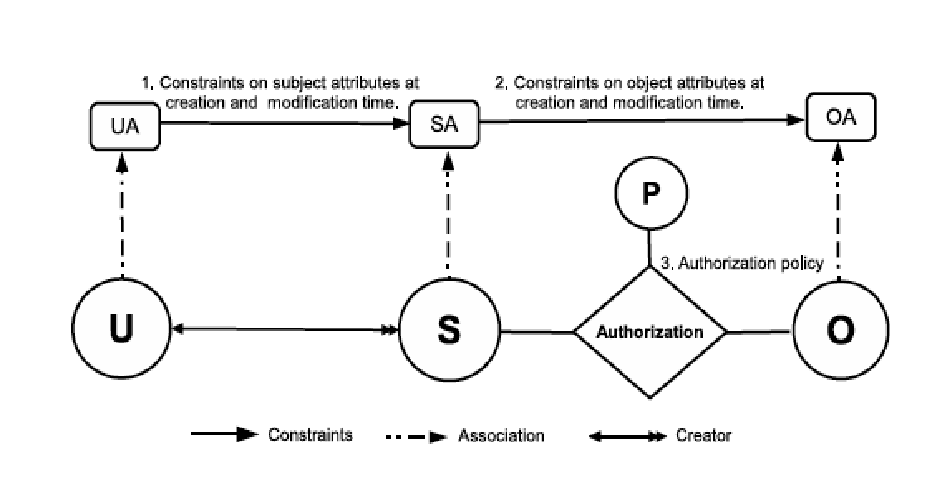
\includegraphics[width=0.3\textwidth]{eps/abac_model}
 \caption{Attribute Based Access Control Model.}
 \label{fig:abac}
\end{figure}

As shown in the diagram,   the authorization policy in this model (shown by the diamond in the figure) is specified with attributes from the subject/users and objects. Without giving any details, we would like to mention that the policy can include any number of user or object attributes.

The interested readers are encouraged to have a look at \cite{abac} where the model components and policy language are discussed in great detail. 


\section{Proposal}

With Swift, the available access control mechanism is  ACL (Access Control List) which specifies who can or cannot access an object or a file. In this approach, if someone can access a document, he/she gets the full content of the document which is an all-or-nothing approach.  Figure \ref{fig:swiftfile} and \ref{fig:zwiftfile}  illustrates the situation where in the former case, a file is accessed in all-or-nothing approach and in the later case the file can be selectively accessed by different users. But we believe that   ZeroVM enables more sophisticated cases which require more flexible access control than the ACL. For example,  a hospital that stores patient medical records in the cloud,  wants all its doctor, nurse or patient access selective content based on the available role of the requester.  So, along with the content, the owner (in this case, the hospital) of an object/file may need to specify who can access how much of the content.

\begin{figure}[h!] 
  \centering
    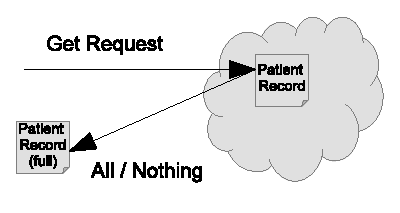
\includegraphics[width=0.3\textwidth]{eps/swift_file}
 \caption{Accessing file with Swift API.}
\label{fig:swiftfile}
\end{figure}

\begin{figure}[h!]
  \centering
    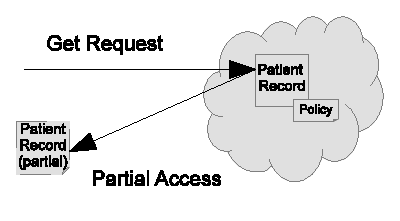
\includegraphics[width=0.3\textwidth]{eps/zwift_file}
 \caption{Our Proposed Solution where file can be accessed selectively}
\label {fig:zwiftfile} 
\end{figure}




Figure  \ref{fig:patient Record}, shows a sample file to be stored in the object store. For our example, we specify following different user roles namely, doctor, patient, nurse and billing stuff.
A sample policy to be specified by the content owner is shown below.

\begin{figure}[h!]
  \centering
    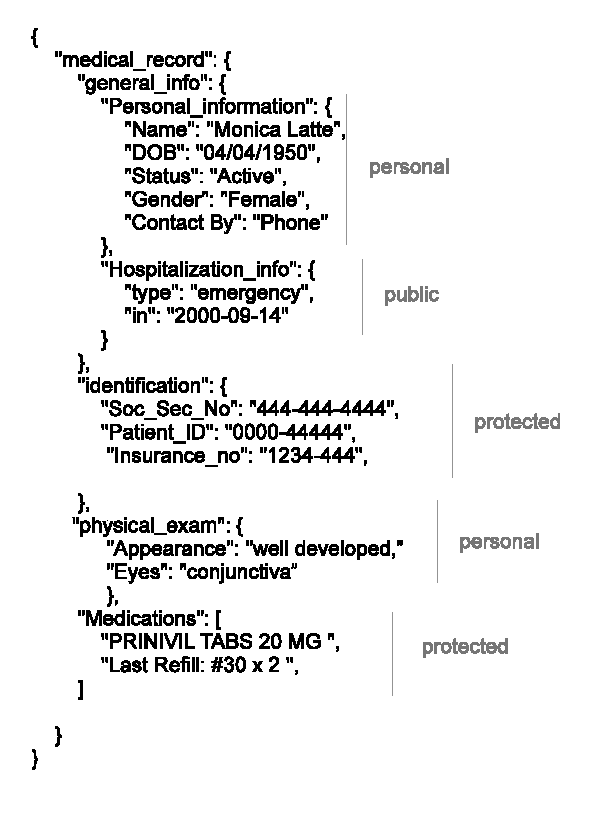
\includegraphics[width=0.3\textwidth]{eps/json-data}
 \caption{Labeled JSON data.}
\label {fig:patient Record} 
\end{figure}



\begin{enumerate}

  \item   Patient own 'personal\_Information' and 'physicalExam' records (see Fig. \ref{fig:patient Record} ). Only the owner can read it.

\item  Patient allow doctor to read her 'physicalExam' records  .
\item  Doctor can read  the entire medical records except information owned by the patient.  
\item  Nurse can read objects identified by  'health\_record'.  
\item  The billing stuffs can only read 'Identification' information.  
\end{enumerate}

In order to  formulate these policy, we would use ABAC (Attribute Based Access Control) model \cite{abac}. In ABAC, user, object is associated with attributes and these attributes are used to specify policies. In \cite{abac}, the authors have provided a simple and easy policy language which is expressive enough to capture Popular Access control models like  DAC( Discretionary Access Control) \cite{dac}, RBAC (Role Based Access Control) \cite{rbac}. To be able to configure DAC and RBAC is important in the sense that the first policy in the above mentioned policies is a DAC policy and the rest are RBAC policies.

In order to specify these policies, we are developing a theoritical work for Access Control model for JSON data where we require user attributes like user role and object attributes like owner and object-label but for the shake of brevity, we are not representing details of the JSON Access Control model  here. Worth to mention that in order to capture user-role we are exploiting the group feature of Identity API version 3 \cite{identityv3}

\begin{figure}[h!]
  \centering
    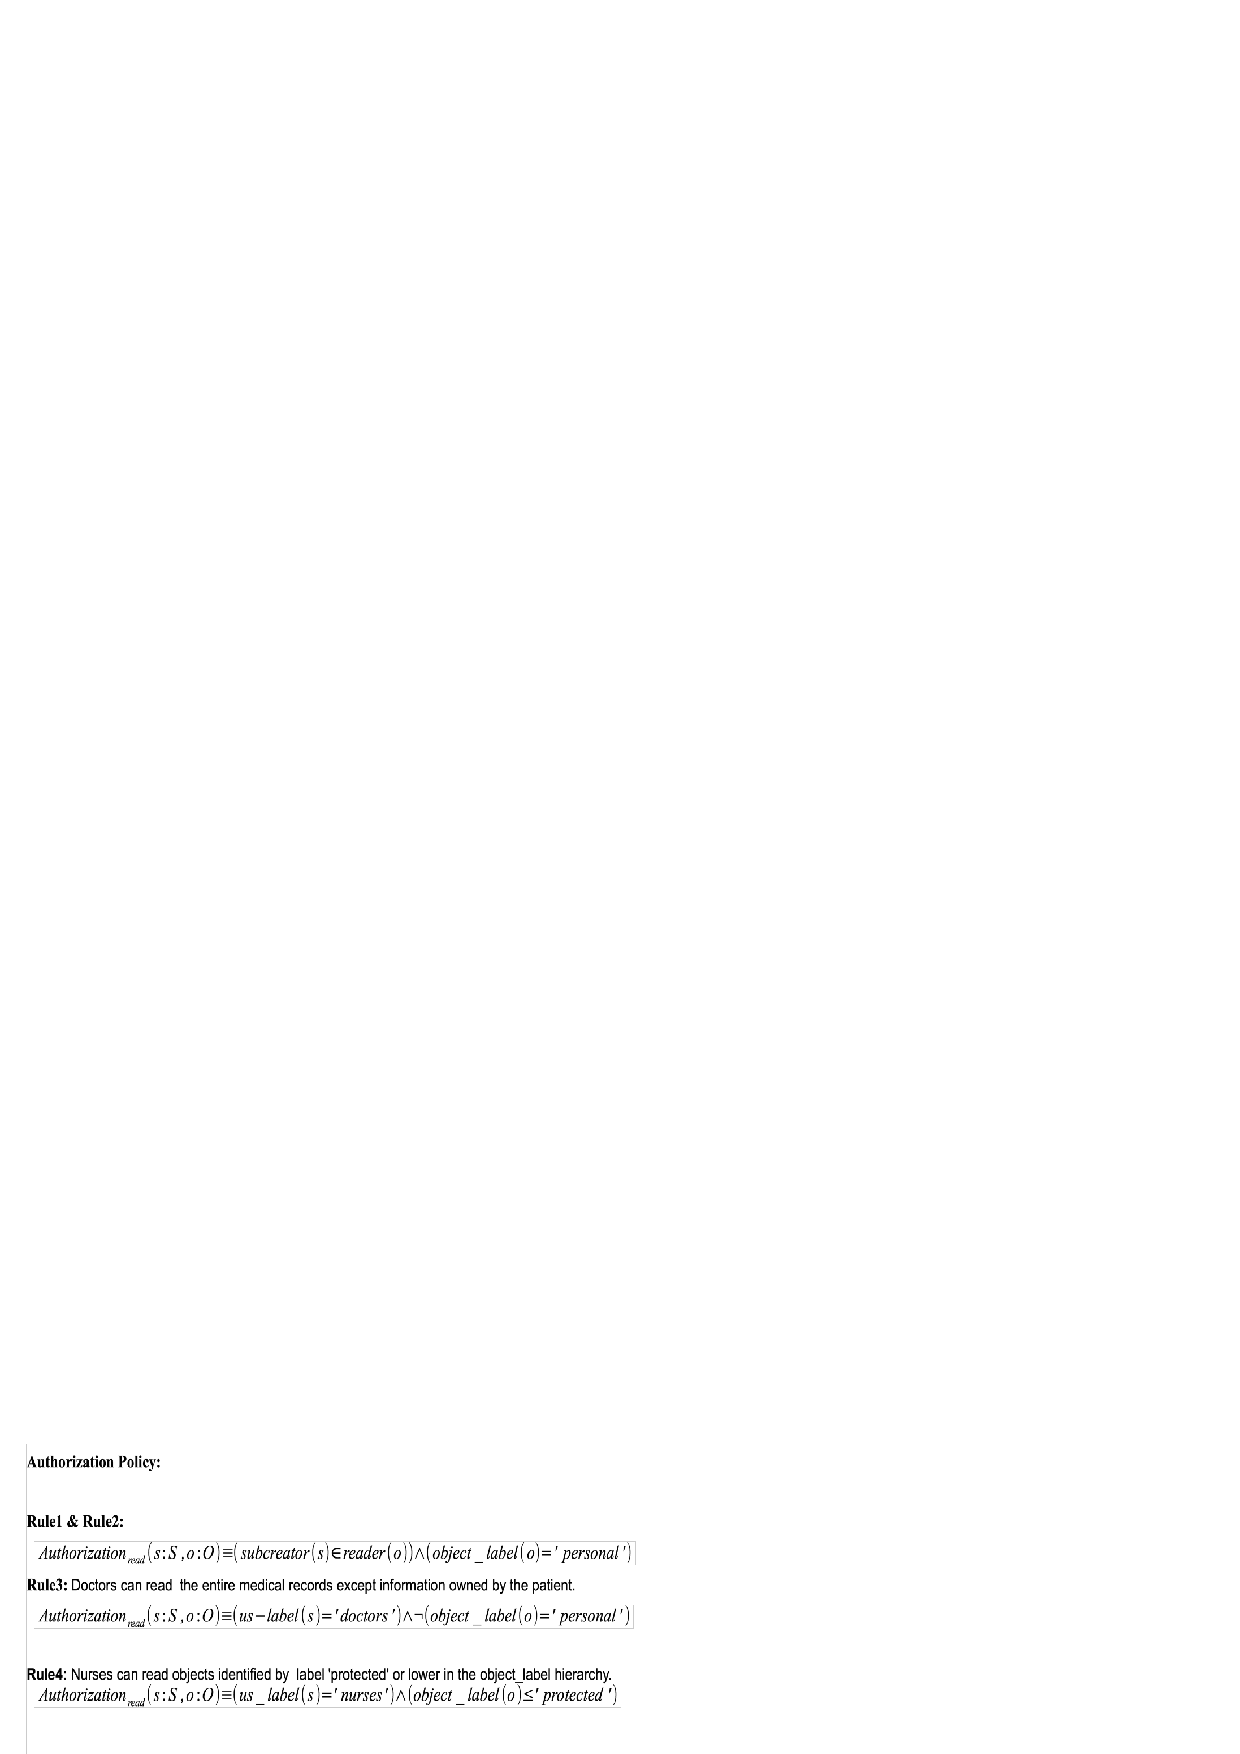
\includegraphics[width=0.5\textwidth]{eps/policy}
 \caption{Configured ABAC policy for given policy.}
\label {fig:policy} 
\end{figure}


Now, whenever a user having role doctor request to get the whole file, he would be able to access only the content as specified in listing \ref{request response} . Figure \ref{fig:policy} shows the configured ABAC policy used in our implementation.

\begin{listing}
\begin{minted}[frame=single,
               framesep=3mm,
               linenos=true,
               xleftmargin=21pt,
               tabsize=2]{js}
{
 "medical_record": { 
      "physical_exam": {
	  "appearance": "well developed",
	  "eyes": "conjunctiva"
	},
  "Medications": [
            "PRINIVIL TABS 20 MG ",
            "Last Refill: #30 x 2 "
        ]   
}  
}

\end{minted}
\caption{Content of  Medical Record Object as Accessed by a User Having Doctor Role} 
\label{request response}
\end{listing}


Again, we envision that it should  be possible to request the file by specifying a JSONPath along with the filename. For example, a requester having role 'doctor' should be able to access only   medication information by specifying a JSON path argument ("//medication") along with the request line. A hypothetical command for the above query would be 

\textbf{ Swift download container patient\_record.json --jsonpath="//medication" }


To sum up our proposal of Content Based Access Control, we want to achieve following:

\begin{figure}[h!] 
  \centering
    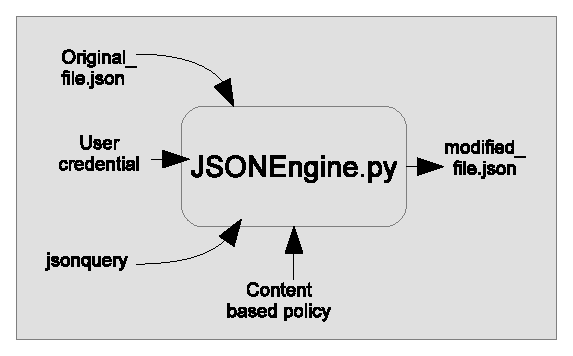
\includegraphics[width=0.3\textwidth]{eps/json_query_zap}
 \caption{The Skeleton for the CBAC zap.}
\label{fig:zappskeleton}
\end{figure}

\begin{enumerate}

  \item Attach policies with a file/object stored in Swift storage. The  file can be requested as it it, or it can be partially requested by specifying query parameter(JSONPath in our case) and instead of having the full content, the requester may get selective content based on his acting role. This case is explained in the above section. The skeleton for the to be developed ZeroVM application is shown in the figure \ref{fig:zappskeleton}



\end{enumerate}










\section { Implementation}

Our implementation does not require any change in the ZeroVM project. We only require following changes in Zerocloud middleware and ZeroVM client program

\begin{enumerate}
\item Changes in the Swift request header
\item Changes in the Zerocloud middleware
\item Changes in the Swift client


\subsection{Request header}
In order to associate policy with the file and specify JSONPath as a query parameter, we need to add two request headers namely, \textbf{--cbac-policy} and \textbf{--jsonpath}.  The values of --cbac-policy header can be a separte policy file or  JSON text specifying the policies. On the otherhand, the value of --jsonpath would be a valid JSONPath. 

\subsection{Zerocloud Middleware}
In the Zerocloud middleware, along with the file to be queried we  need to capture the values of --cbac-policy ( or retrieve corresponding policy file). We may need to modify the ZeroVM manifest file to include this policy file as another valid input channel. 

\subsection{ZeroVM client}

In order to specify --cbac-policy and --jsonpath headers, we may need to modify python-swiftclient or zpm command.

\end{enumerate}
\section{Conclusion}
As more and more data is being uploaded in the cloud, these data may contain sensitive information. With existing swift API, one can either access the full content or nothing. We have presented somelegitimate situations where one should be given access to a  file with sensitive content being filtered out.  With the coupling of swift with zerovm, we are proposing here to develop an application where someone can specify policy with a file and let different user access different parts of it. Currenly, our content based access control is limited to one file, but it the future we want to implement it for multiple linked files.





\section*{Acknowledgment}


The authors would like to thank RackSpace, the open cloud company for supporting this project.






\begin{thebibliography}{1}

  \bibitem{abac} Xin Jin, Ram Krishnan, Ravi Sandhu  {\em A Unified Attribute-Based Access Control Model Covering DAC, MAC and RBAC}  2012.
   \bibitem{dac} Sandhu, Ravi S., and Pierangela Samarati. {\em Access control: principle and practice.} Communications Magazine, IEEE 32.9 (1994): 40-48.
   
 \bibitem{rbac} Sandhu, Ravi S., et al. {\em Role-based access control models.} Computer 29.2 (1996): 38-47.  
   

  \bibitem{zerovm}    {\em ZeroVM}  available at : http://zerovm.org/   
  
  \bibitem{nacl}    {\em Google Native Client }  available at : json.org
  
    \bibitem{json}    {\em JSON }  available at : https://code.google.com/p/nativeclient/
    
 \bibitem{mongodb}    {\em mongodb}  available at : http://docs.mongodb.org/manual/
 
  \bibitem{abacwiki}    {\em Google Native Client }  available at : http://en.wikipedia.org/wiki/Attribute\_Based\_Access\_Control

\bibitem{identityv3}    {\em OpenStack Identity API V3}  available at : http://developer.openstack.org/api-ref-identity-v3.html 
  
  \bibitem{zpm}    {\em ZeroVM Package manager }  available at : http://zerovm-zpm.readthedocs.org/en/latest/
  
    \bibitem{docker}    {\em Docker }  available at : http://www.docker.com/
    




  \end{thebibliography}



% that's all folks
\end{document}


